\documentclass[tikz,border=10pt]{standalone}
\usetikzlibrary{calc}
\begin{document}
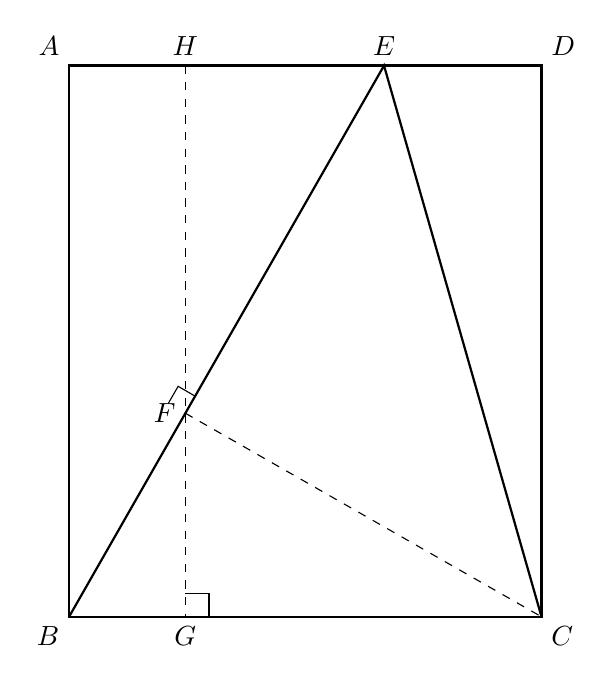
\begin{tikzpicture}[scale=1]
\coordinate (A) at (0,7);
\coordinate (B) at (0,0);
\coordinate (C) at (6,0);
\coordinate (D) at (6,7);
\coordinate (E) at (4,7);
\coordinate (H) at (1.477,7);
\coordinate (G) at (1.477,0);
\coordinate (F) at (1.477,2.585);

\draw[thick] (A) -- (B) -- (C) -- (D) -- cycle;
\draw[thick] (B) -- (E) -- (C);
\draw[dashed] (H) -- (G);
\draw[dashed] (F) -- (C);

% right angle mark at G
\draw ($(G)+(0,0.3)$) -- ($(G)+(0.3,0.3)$) -- ($(G)+(0.3,0)$);
% right angle mark at F (between FE and FC)
\draw[rotate around={60:(F)}] ($(F)+(0,0.25)$) -- ($(F)+(0.25,0.25)$) -- ($(F)+(0.25,0)$);

\node[above left] at (A) {$A$};
\node[below left] at (B) {$B$};
\node[below right] at (C) {$C$};
\node[above right] at (D) {$D$};
\node[above] at (E) {$E$};
\node[above] at (H) {$H$};
\node[below] at (G) {$G$};
\node[left] at (F) {$F$};
\end{tikzpicture}
\end{document}
